\section{Alternative Analyses}

Two alternative analyses were implemented in order to provide a cross-check of the 
modelling for the V+jets backgrounds described in section~\ref{sec:zjetsmodel}. 
For both analyses the selection and categorisation of the events 
are identical to the baseline analysis. In addition, the definitions of the control regions 
are also that used for the baseline analysis. All of the systematics described in the main text 
are also included in both analyses, though their effect is re-evaluated for each alternative analysis. 

\subsubsection{Parametric analysis}

In order to further constrain the tails of the distributions of \ETm in the V+jets backgrounds, the low and high ends 
of the spectrum can be correlated through the use of a parametric function. In this analysis, the high statistics 
of the lower \ETm events is exploited and the shape extrapolated to the high \ETm events. 
The \ETm distributions of the \Zvvjets~events and \Wlvjets~events in the signal region are parameterized as the sum of two exponential functions in the 
monojet category whereas for the boosted and resolved categories, due to the lower statistics 
in these categories, a single power law is used. An unbinned fit of these functions is first performed to the simulated Z+jets or W+jets events 
in the signal region.
Taking one event category, for each bin in fake \ETm, the number of expected events in each of the three 
control regions can be expressed as, 
\begin{equation}
N^{Z_{\mu\mu}/\gamma }_{i} (\boldsymbol{\alpha})=  \dfrac{1}{R^{Z/\gamma}_{i}} \int_{\mathrm{Bin_i}} f(\boldsymbol{\alpha},\ETm),
\end{equation} 
for the dimuon and photon plus jet control regions and,
\begin{equation}
N^{W}_{i}(\boldsymbol{\beta}) =  \dfrac{1}{R^{W}_{i}} \int_{\mathrm{Bin_i}} g(\boldsymbol{\beta},\ETm),
\end{equation} 
for the single muon control region, where $\boldsymbol{\alpha}$ and $\boldsymbol{\beta}$ are the free parameters 
of the double exponential or power law functions used to parameterize the\ETm spectrum of the 
 $\Zvvjets$ ($f$) and $\Wlvjets$ ($g$) backgrounds.
 The likelihood for each category then becomes,

\begin{align*}
\mathcal{L}_{\textrm{c}}(\boldsymbol{\alpha}^{\textrm{c}}\boldsymbol{\beta}^{\textrm{c}},\boldsymbol{\theta},\boldsymbol{\phi}) &=        
                \prod_{i} \mathrm{Possion}(d^{\textrm{c},\gamma}_{i} |B^{\textrm{c},\gamma}_{i}(\boldsymbol{\phi}) +\int_{\mathrm{bin}_{i}} \frac{1}{R^{\textrm{c},\gamma}_{i}(\boldsymbol{\theta})} f^{\textrm{c}}(\boldsymbol{\alpha}^{c},E_{T}^{miss})   ) \\
       &~\times \prod_{i} \mathrm{Possion}(d^{\textrm{c},Z}_{i}      |B^{\textrm{c},Z}_{i}(\boldsymbol{\phi})      +\int_{\mathrm{bin}_{i}} \frac{1}{R^{\textrm{c},Z}_{i}(\boldsymbol{\theta})} f^{\textrm{c}}(\boldsymbol{\alpha}^{c},E_{T}^{miss})        ) \\
       &~\times \prod_{i} \mathrm{Possion}(d^{\textrm{c},W}_{i}     |B^{\textrm{c},W}_{i}(\boldsymbol{\phi})      +\int_{\mathrm{bin}_{i}} \frac{1}{R^{\textrm{c},W}_{i}(\boldsymbol{\theta})} g^{\textrm{c}}(\boldsymbol{\beta}^{c},E_{T}^{miss})        ) \\
\end{align*}
where the constrained nuisance parameters $\boldsymbol{\theta}$ and $\boldsymbol{\phi}$ are the same as in the 
baseline analysis and the superscript ``c'' indicates components uncorrelated between categories.
The full likelihood is again a product of $\mathcal{L}_{\textrm{c}}$ over the three event categories.

As with the baseline analysis, the likelihood is maximised (fit) with respect to the parameters, this time being 
those of the parametric function, $\boldsymbol{\alpha}^{c}$ and $\boldsymbol{\beta}^{c}$  
 and the nuisance parameters. 
The ratio of the functions $f^{\textrm{c}}(\ETm)$ and $g^{\textrm{c}}(\ETm)$ at the values of the parameters which maximise the 
likelihood to that before the fit provides a correction as a function of \ETm which can be used to re-weight the Z+jets and W+jets simulation in the 
signal region. The results of the fit are shown in 
Figure~\ref{fig:combined_fit_result_mbin}.

\begin{figure*}[hbtp]\begin{center}
 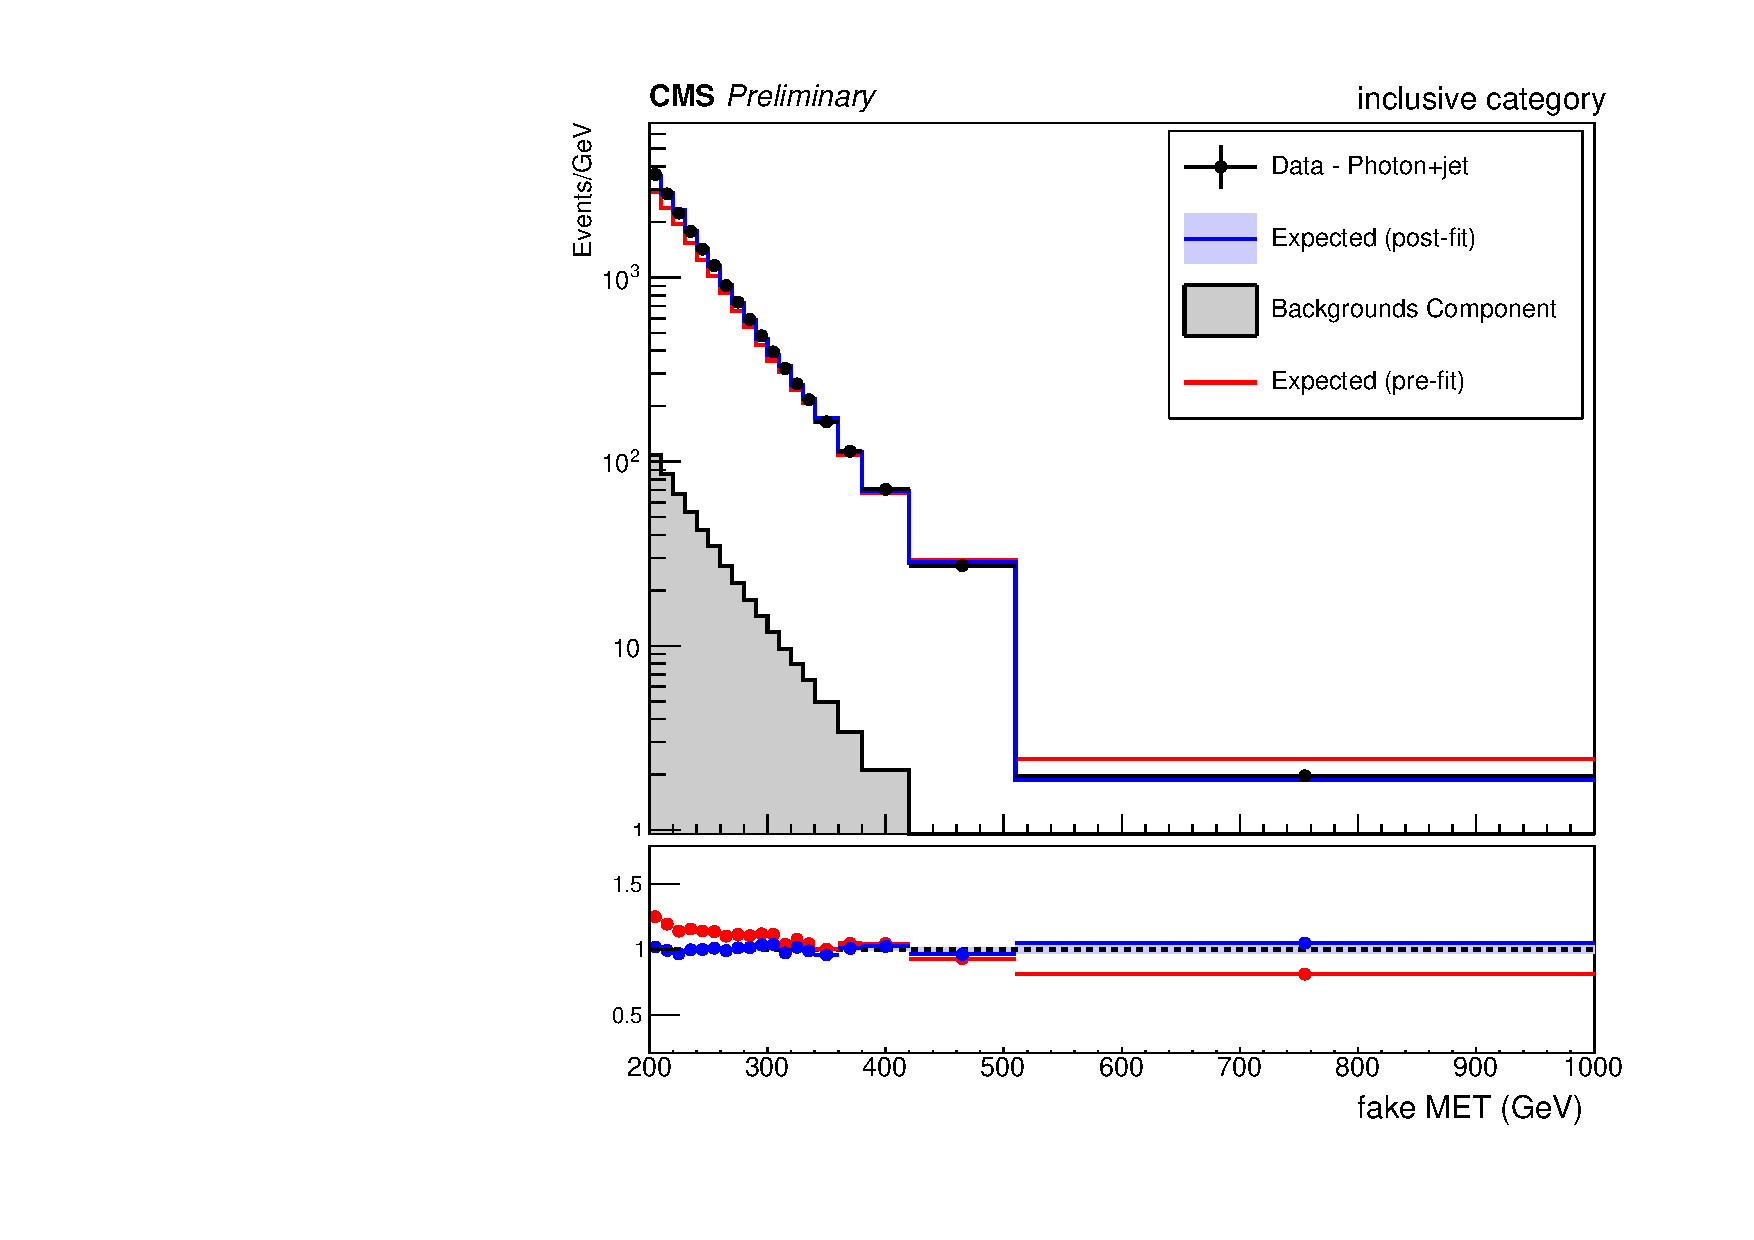
\includegraphics[width=0.32\textwidth]{fig/post_fit_photon_inclusive.pdf}
 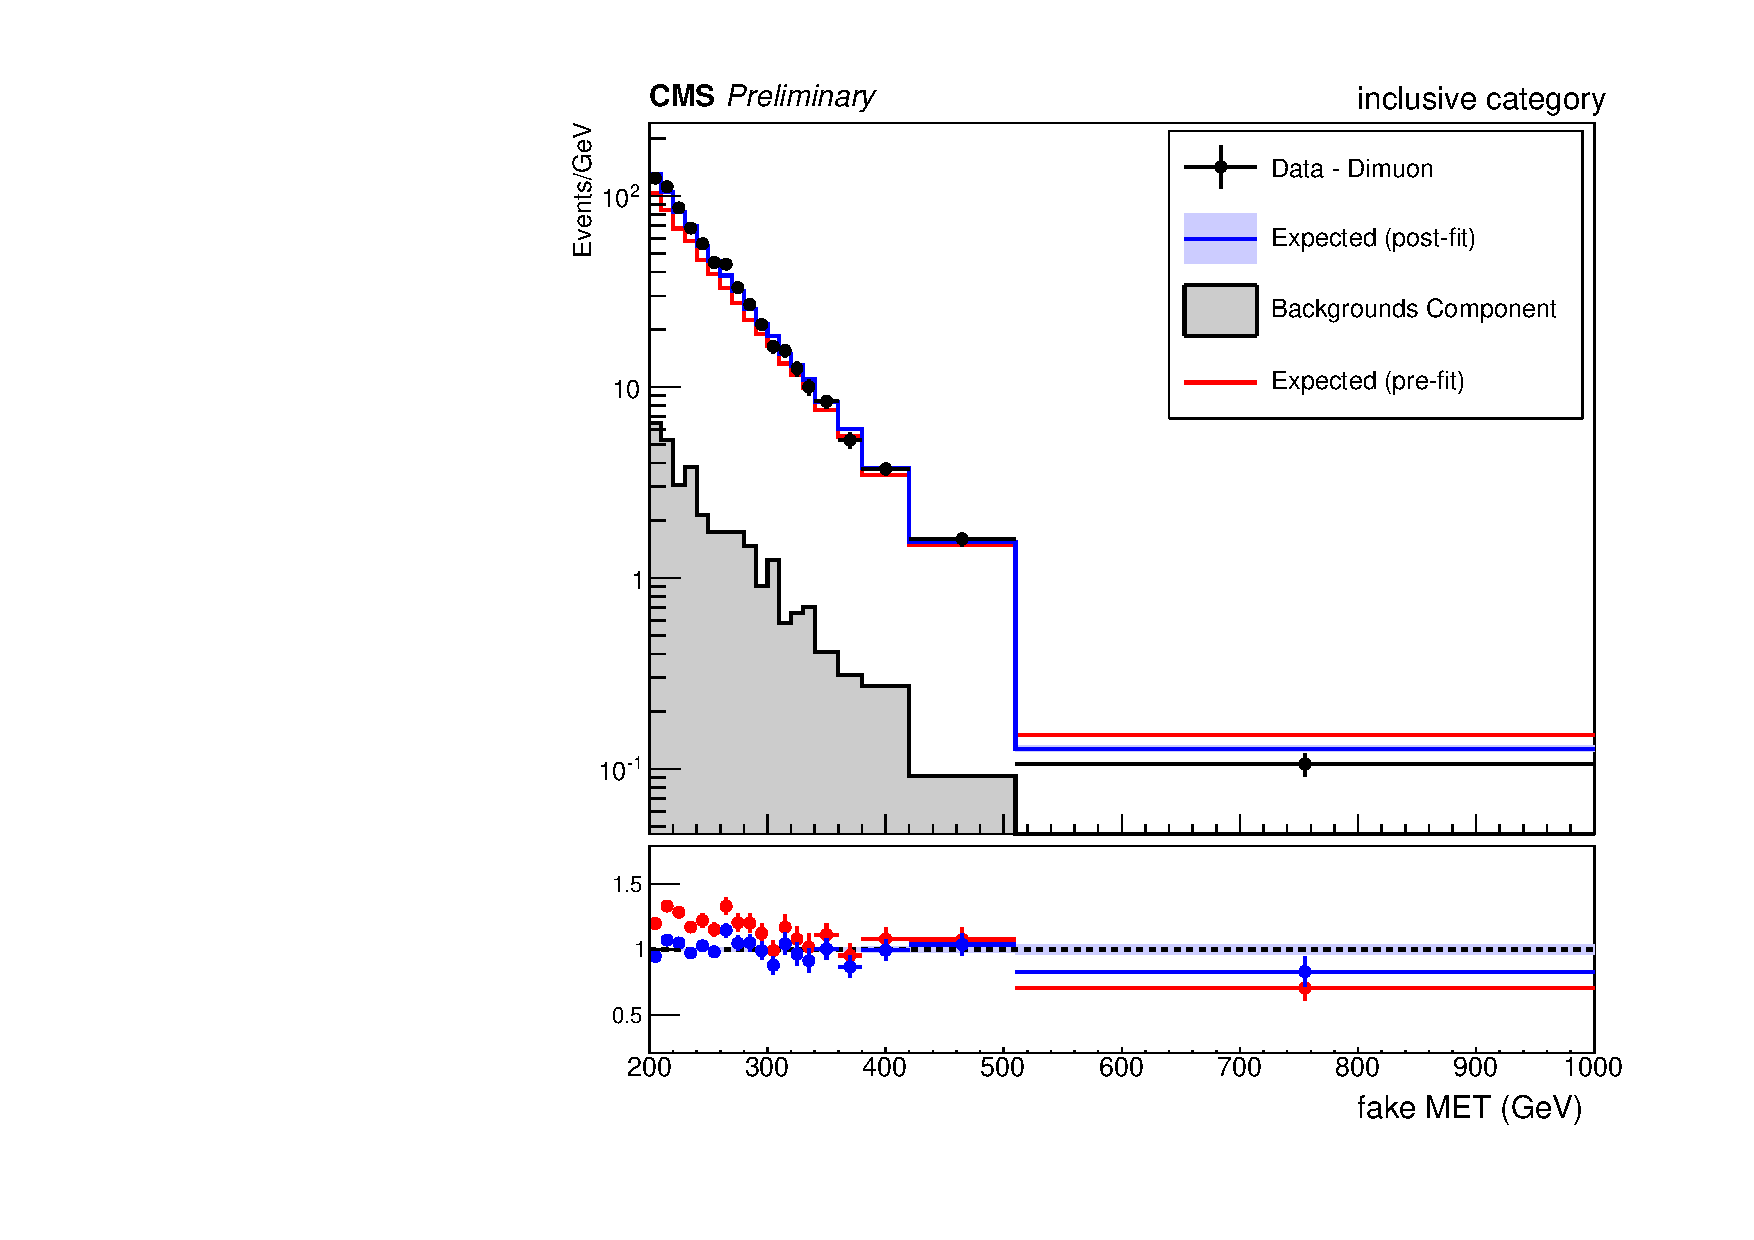
\includegraphics[width=0.32\textwidth]{fig/post_fit_zmm_inclusive.pdf}
 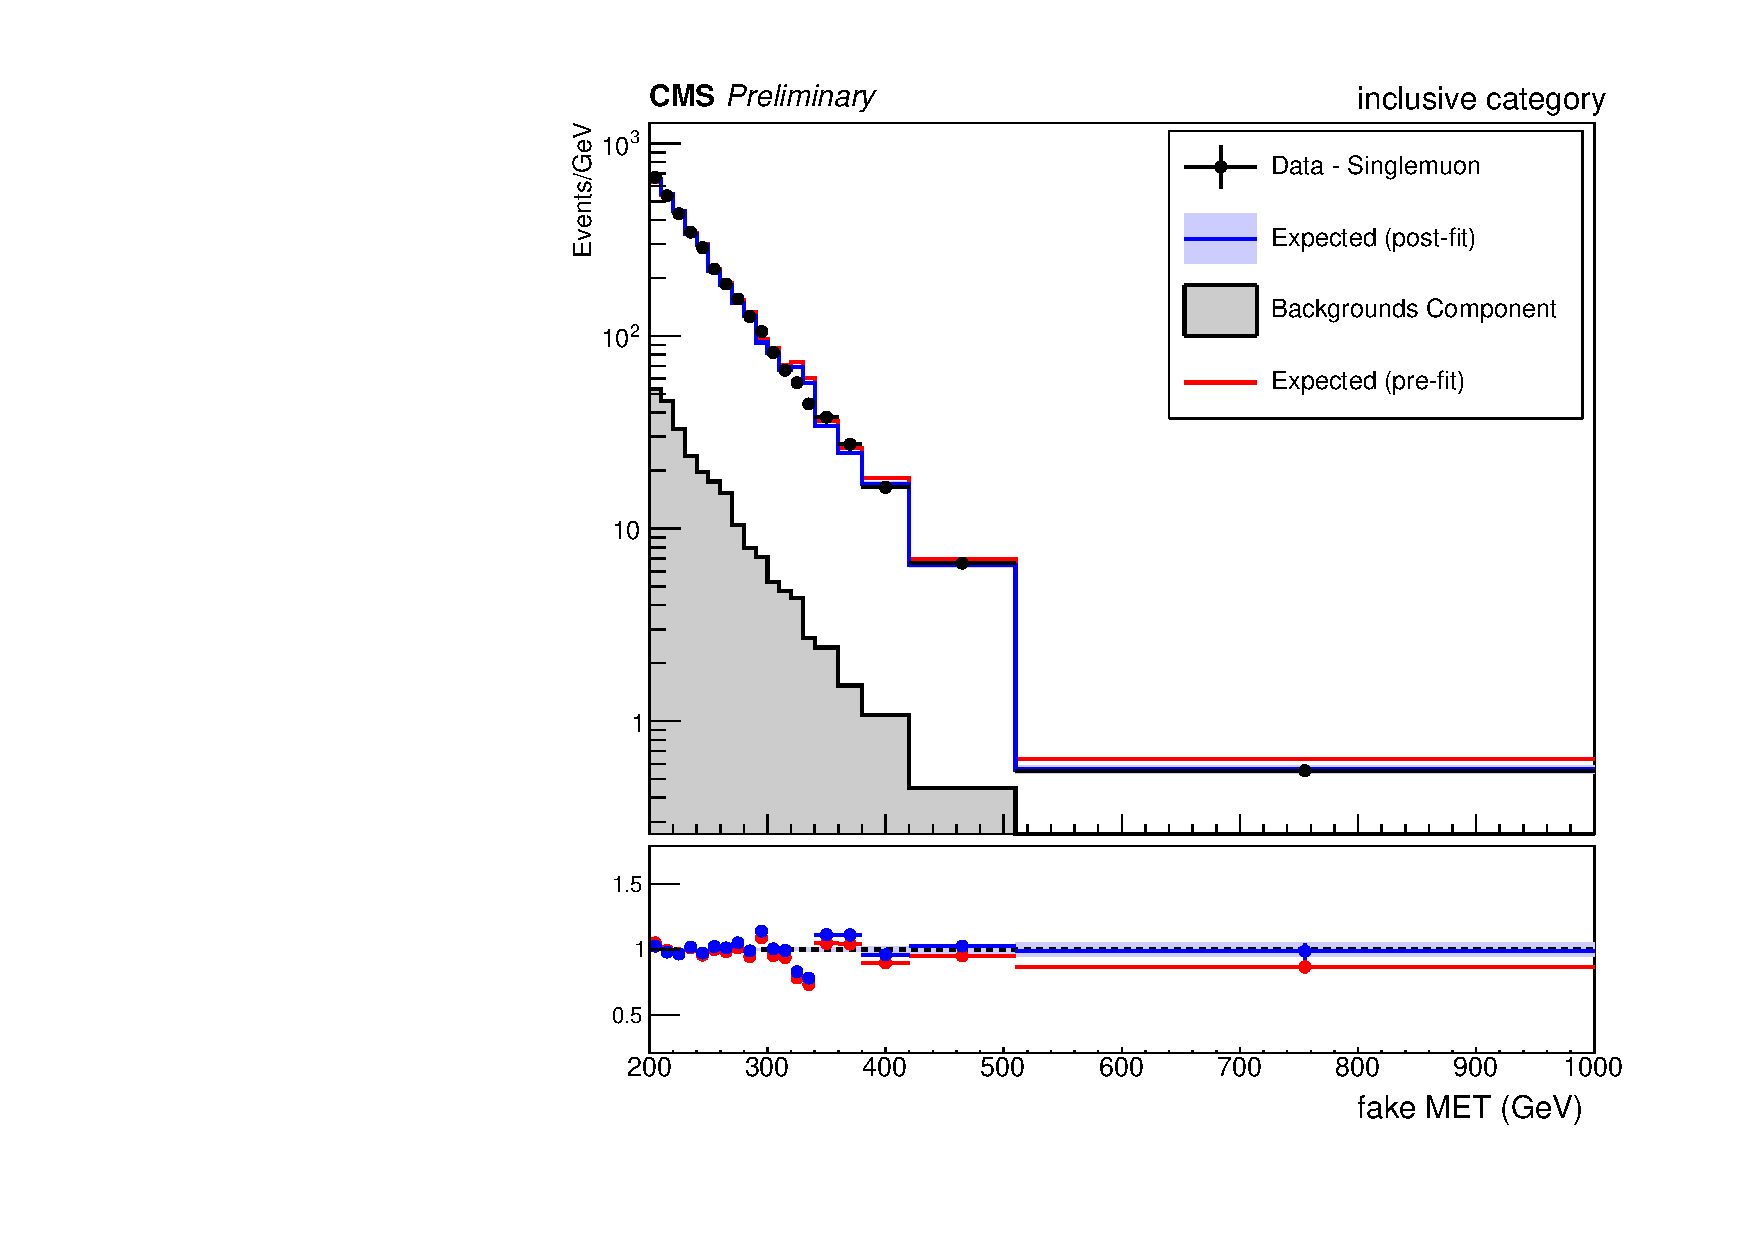
\includegraphics[width=0.32\textwidth]{fig/post_fit_wmn_inclusive.pdf}\\
 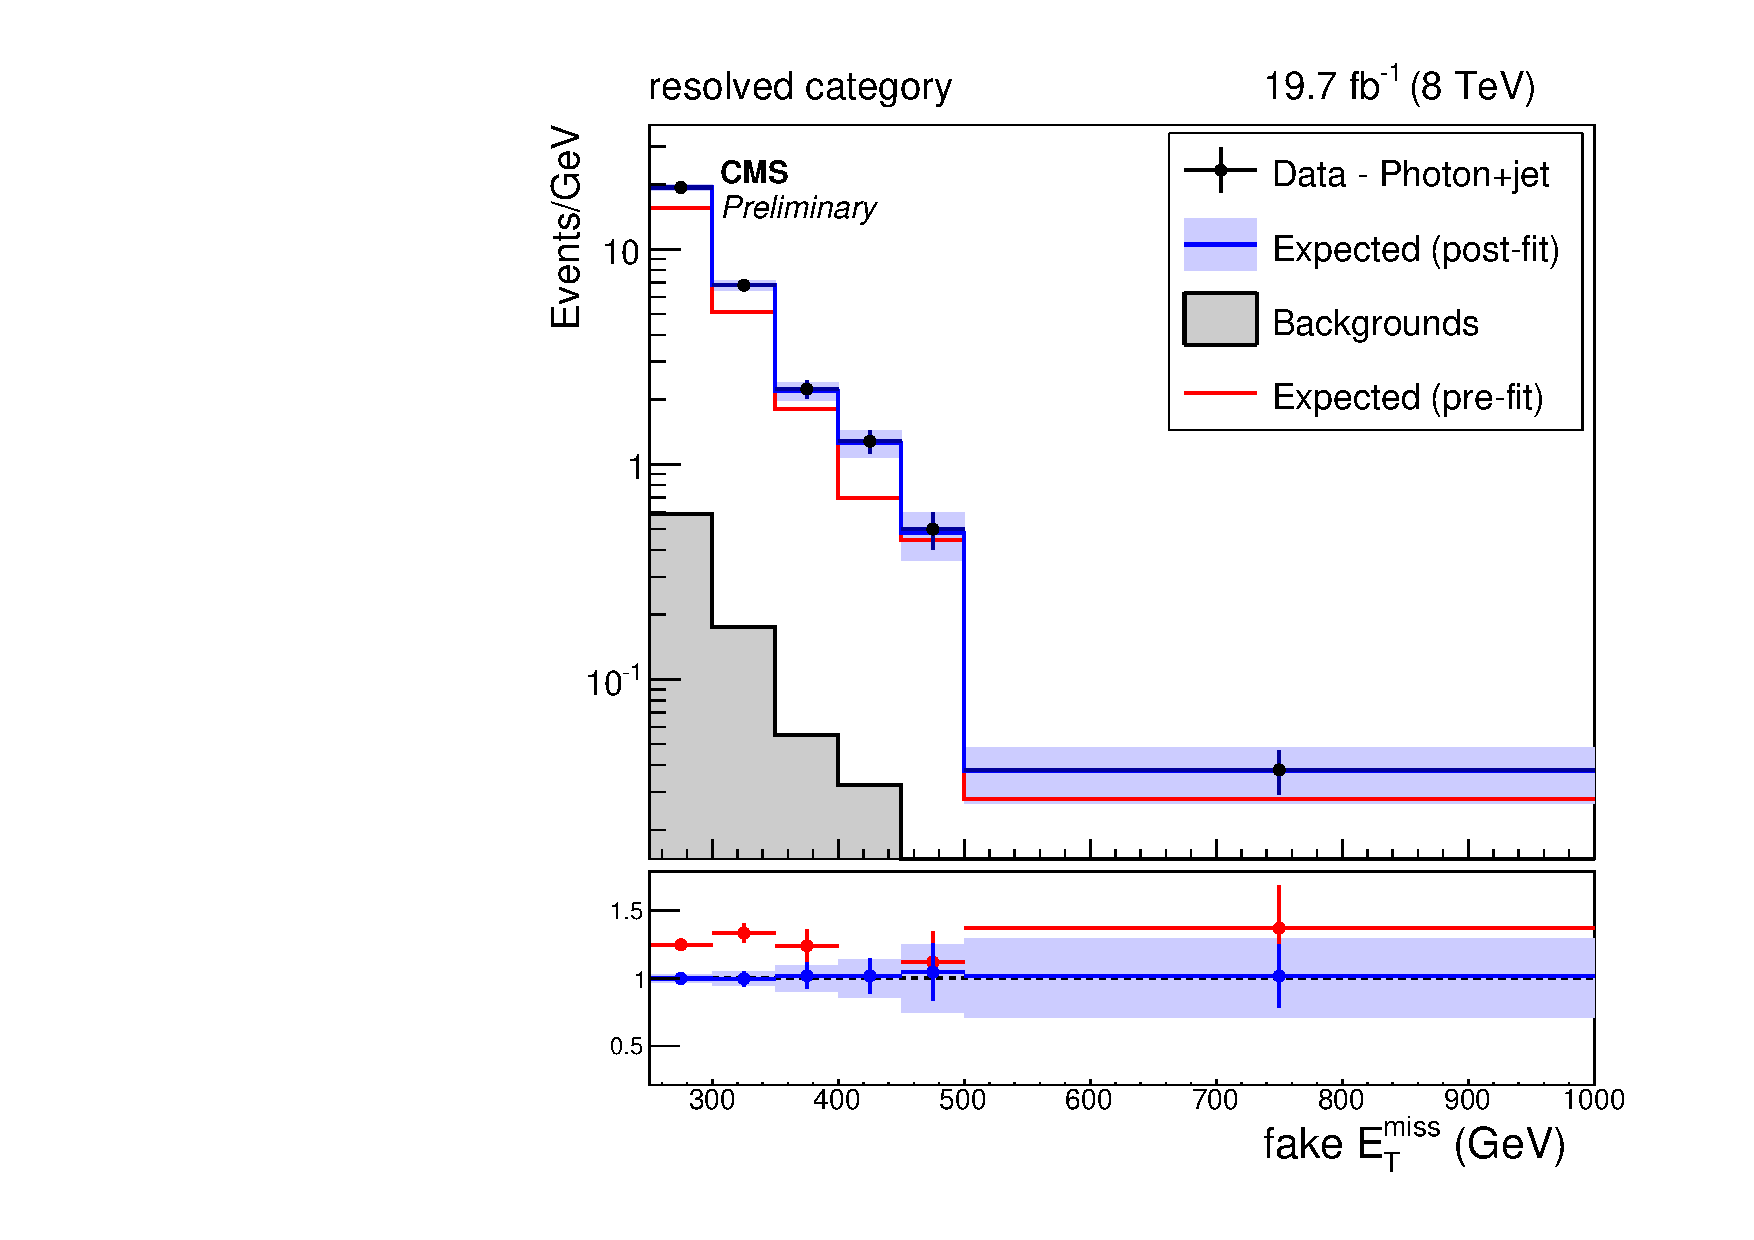
\includegraphics[width=0.32\textwidth]{fig/post_fit_photon_resolved.pdf}
 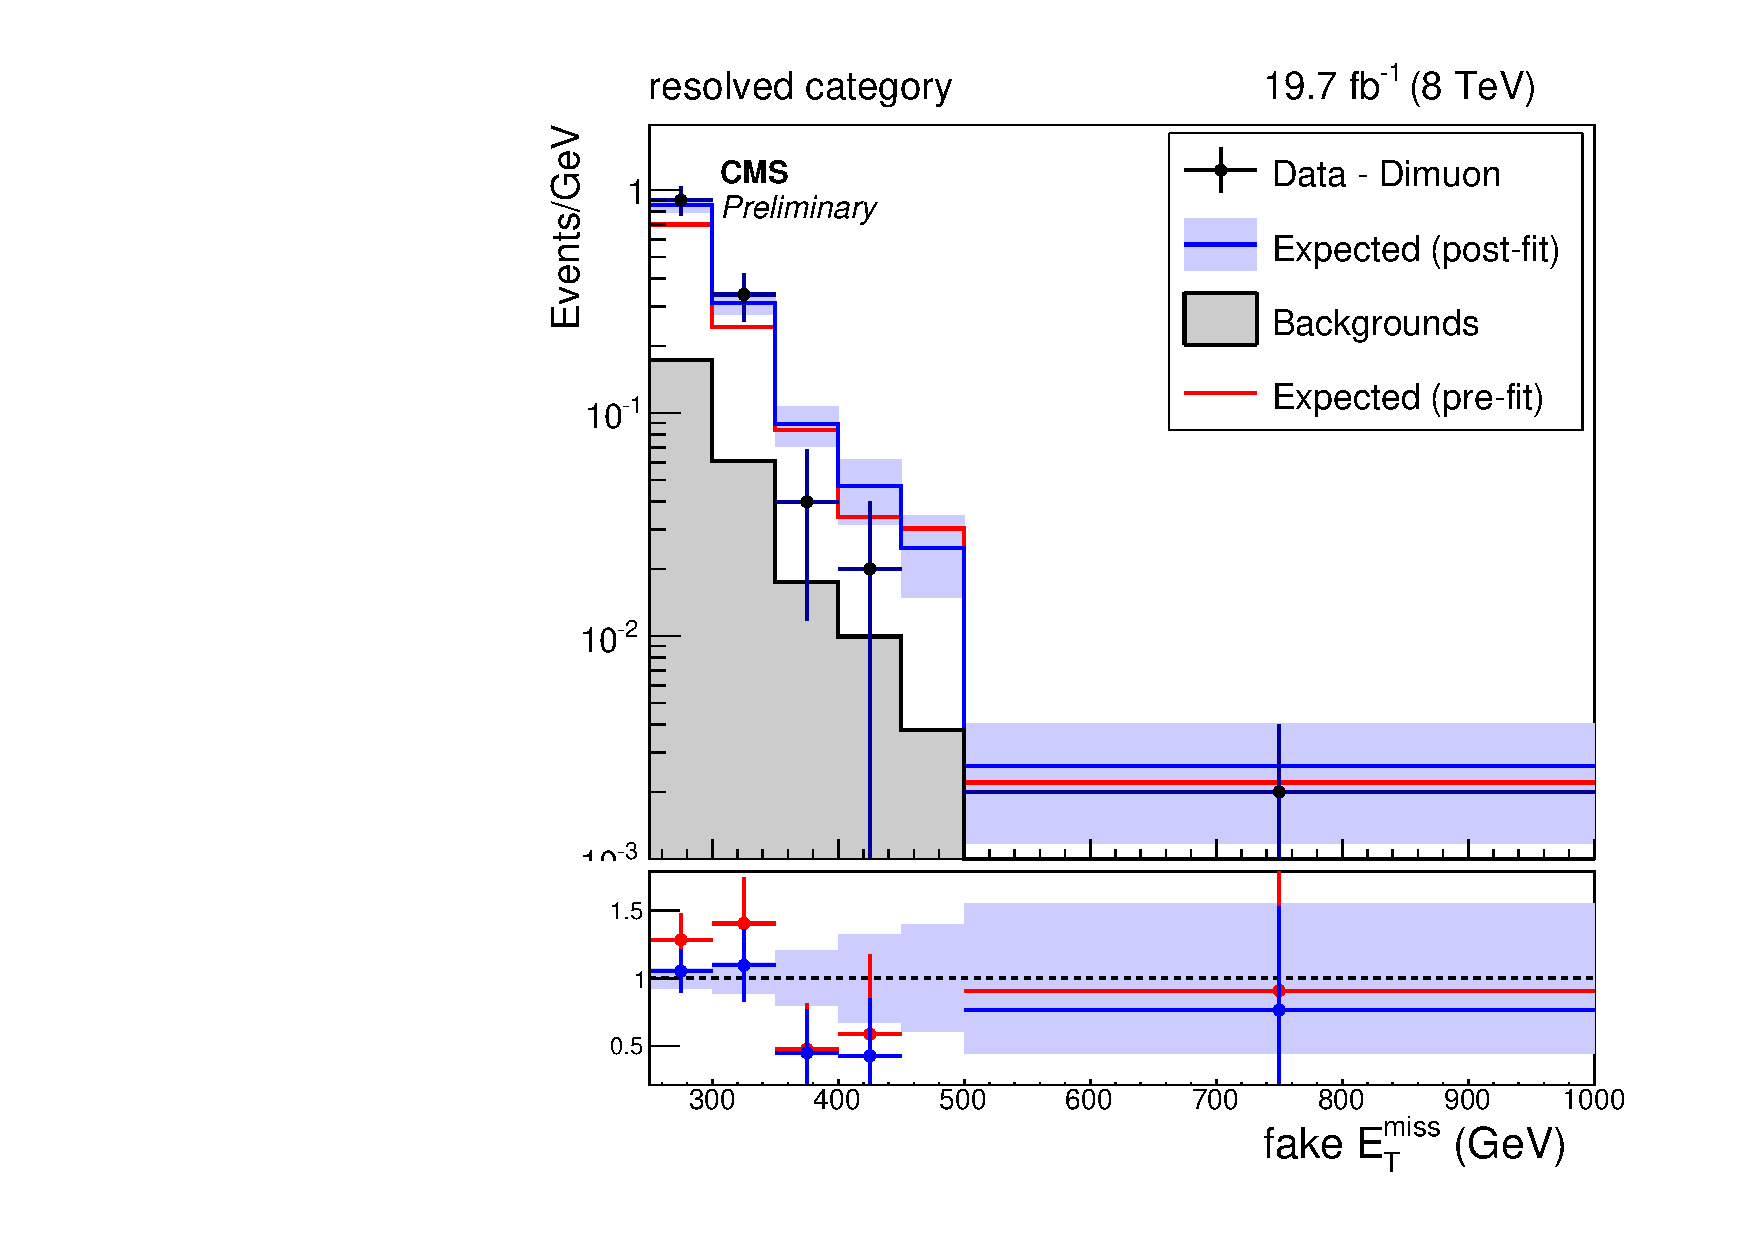
\includegraphics[width=0.32\textwidth]{fig/post_fit_zmm_resolved.pdf}
 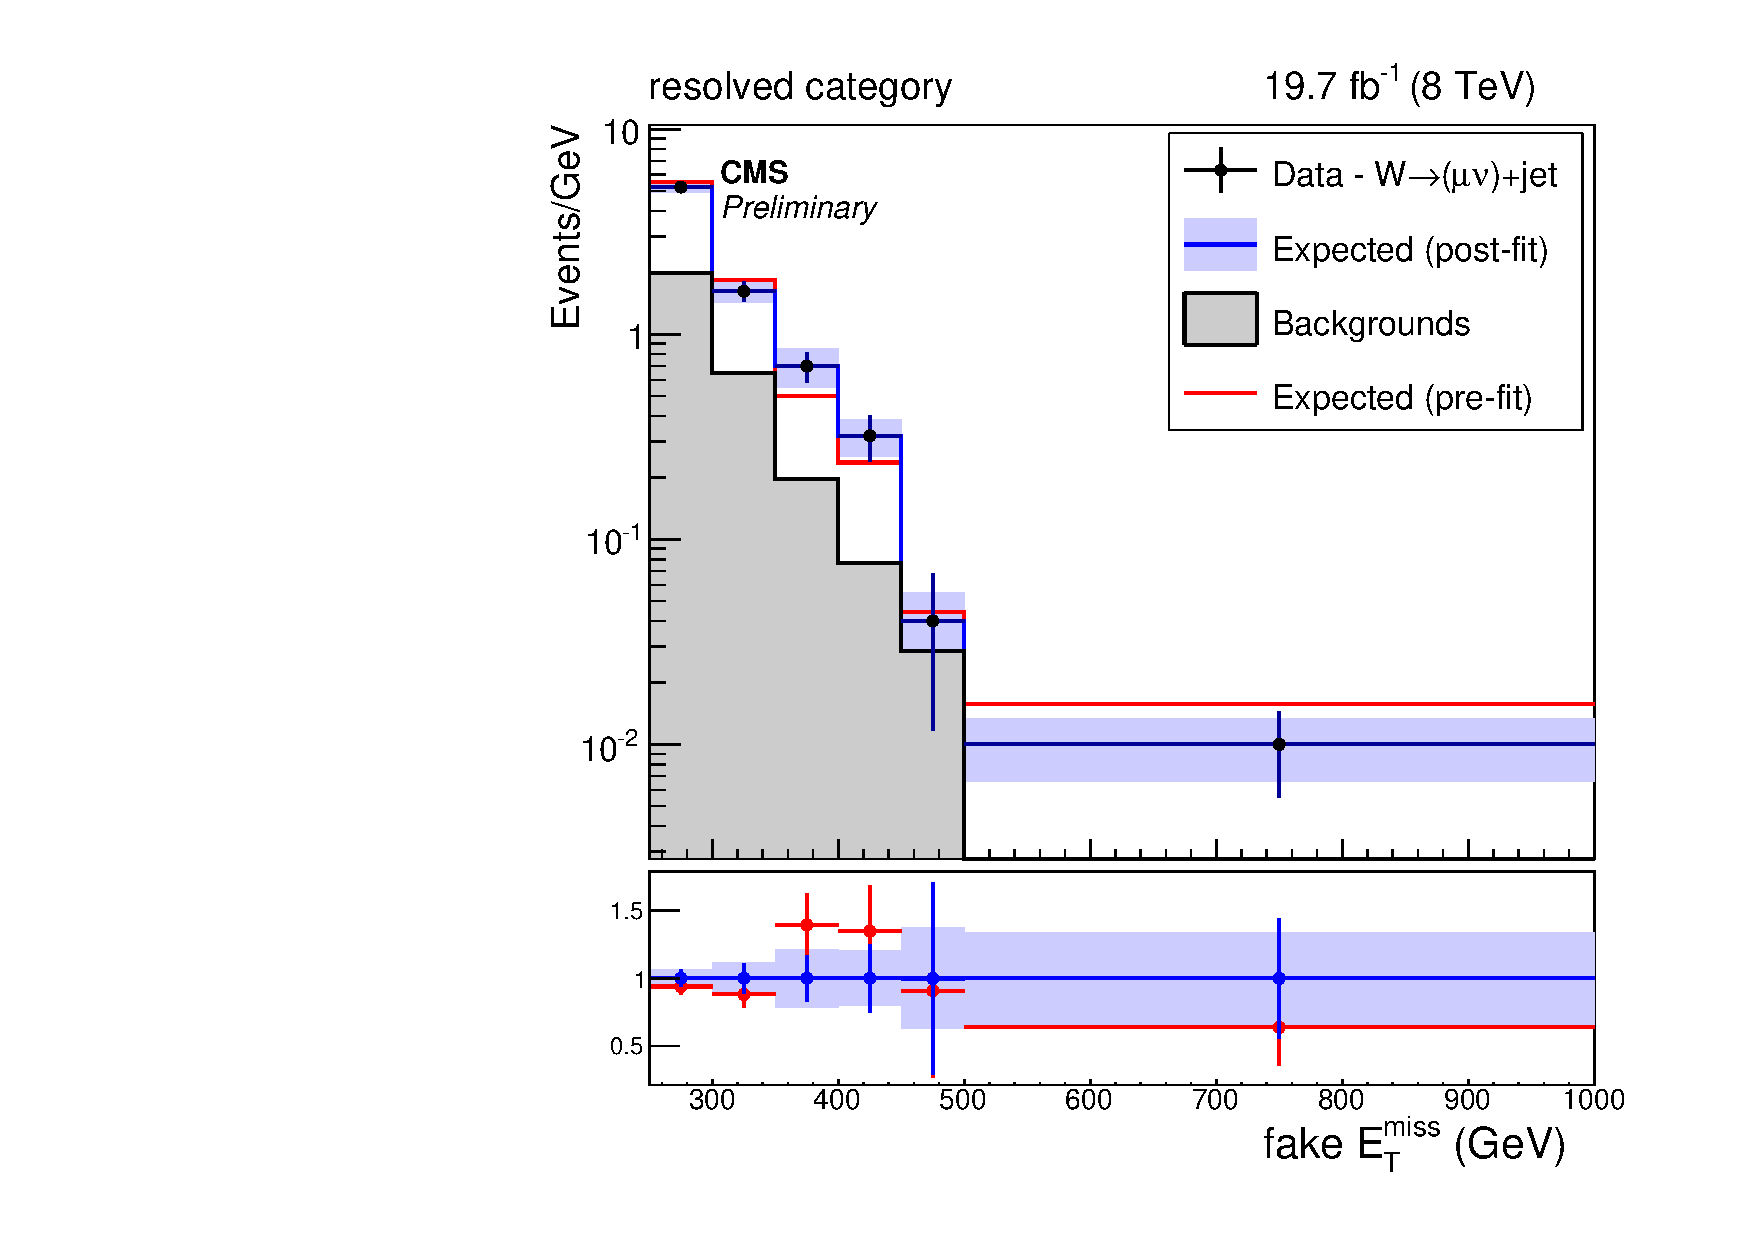
\includegraphics[width=0.32\textwidth]{fig/post_fit_wmn_resolved.pdf}\\
 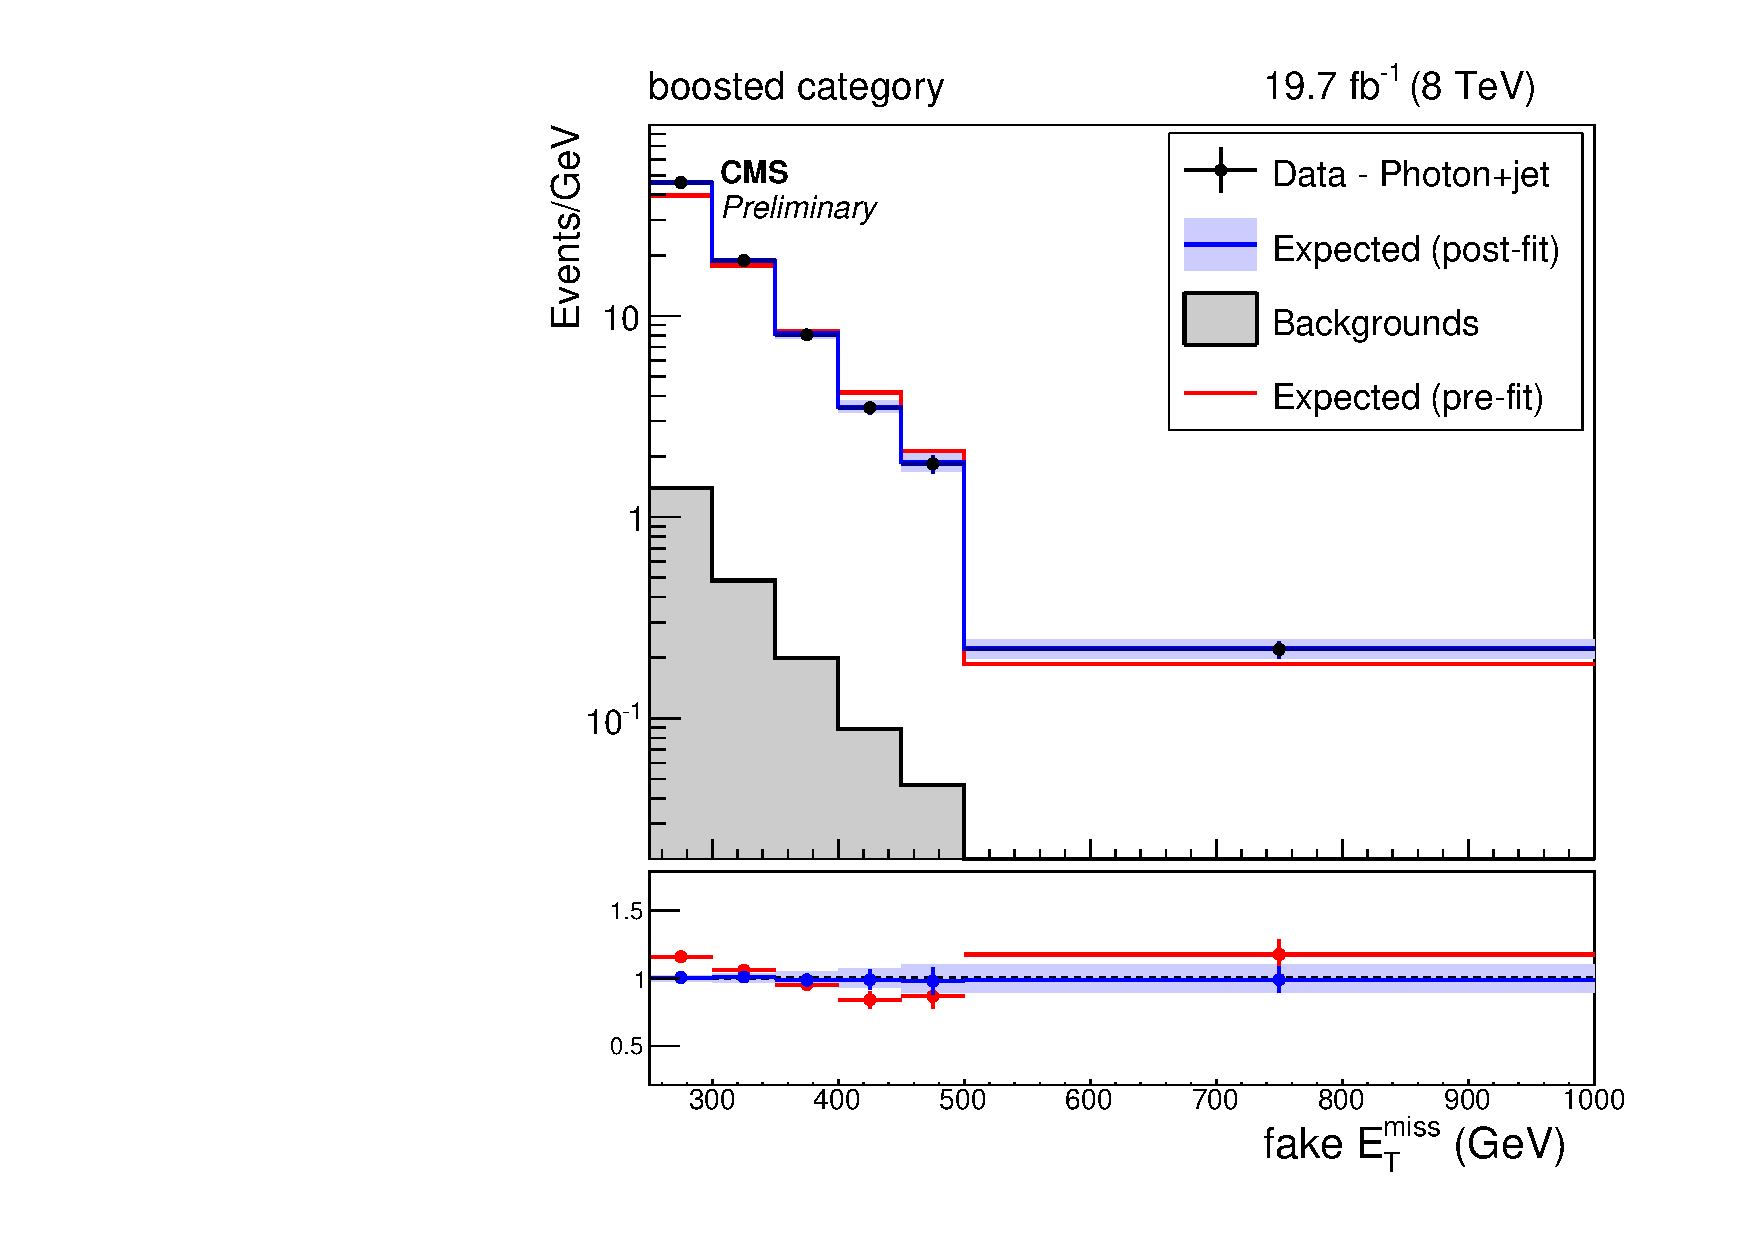
\includegraphics[width=0.32\textwidth]{fig/post_fit_photon_boosted.pdf}
 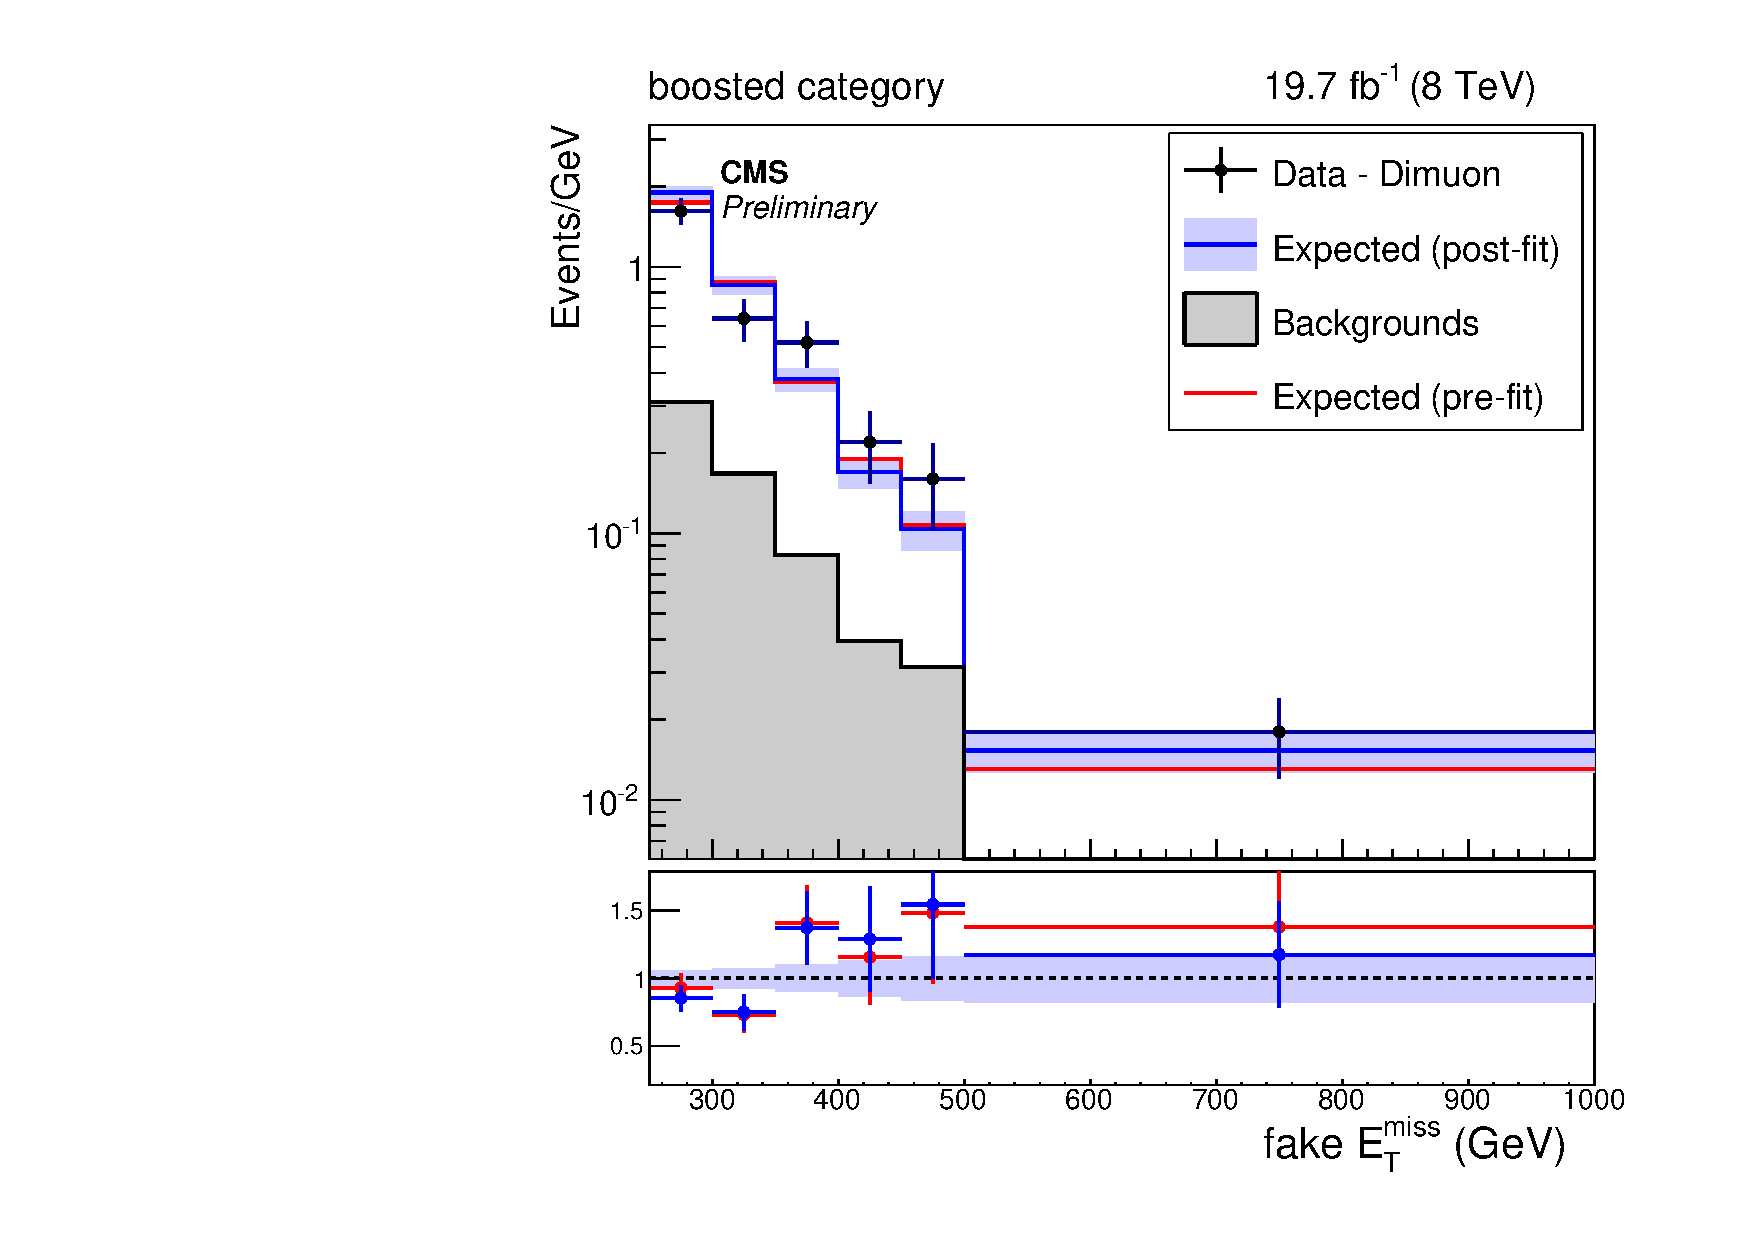
\includegraphics[width=0.32\textwidth]{fig/post_fit_zmm_boosted.pdf}
 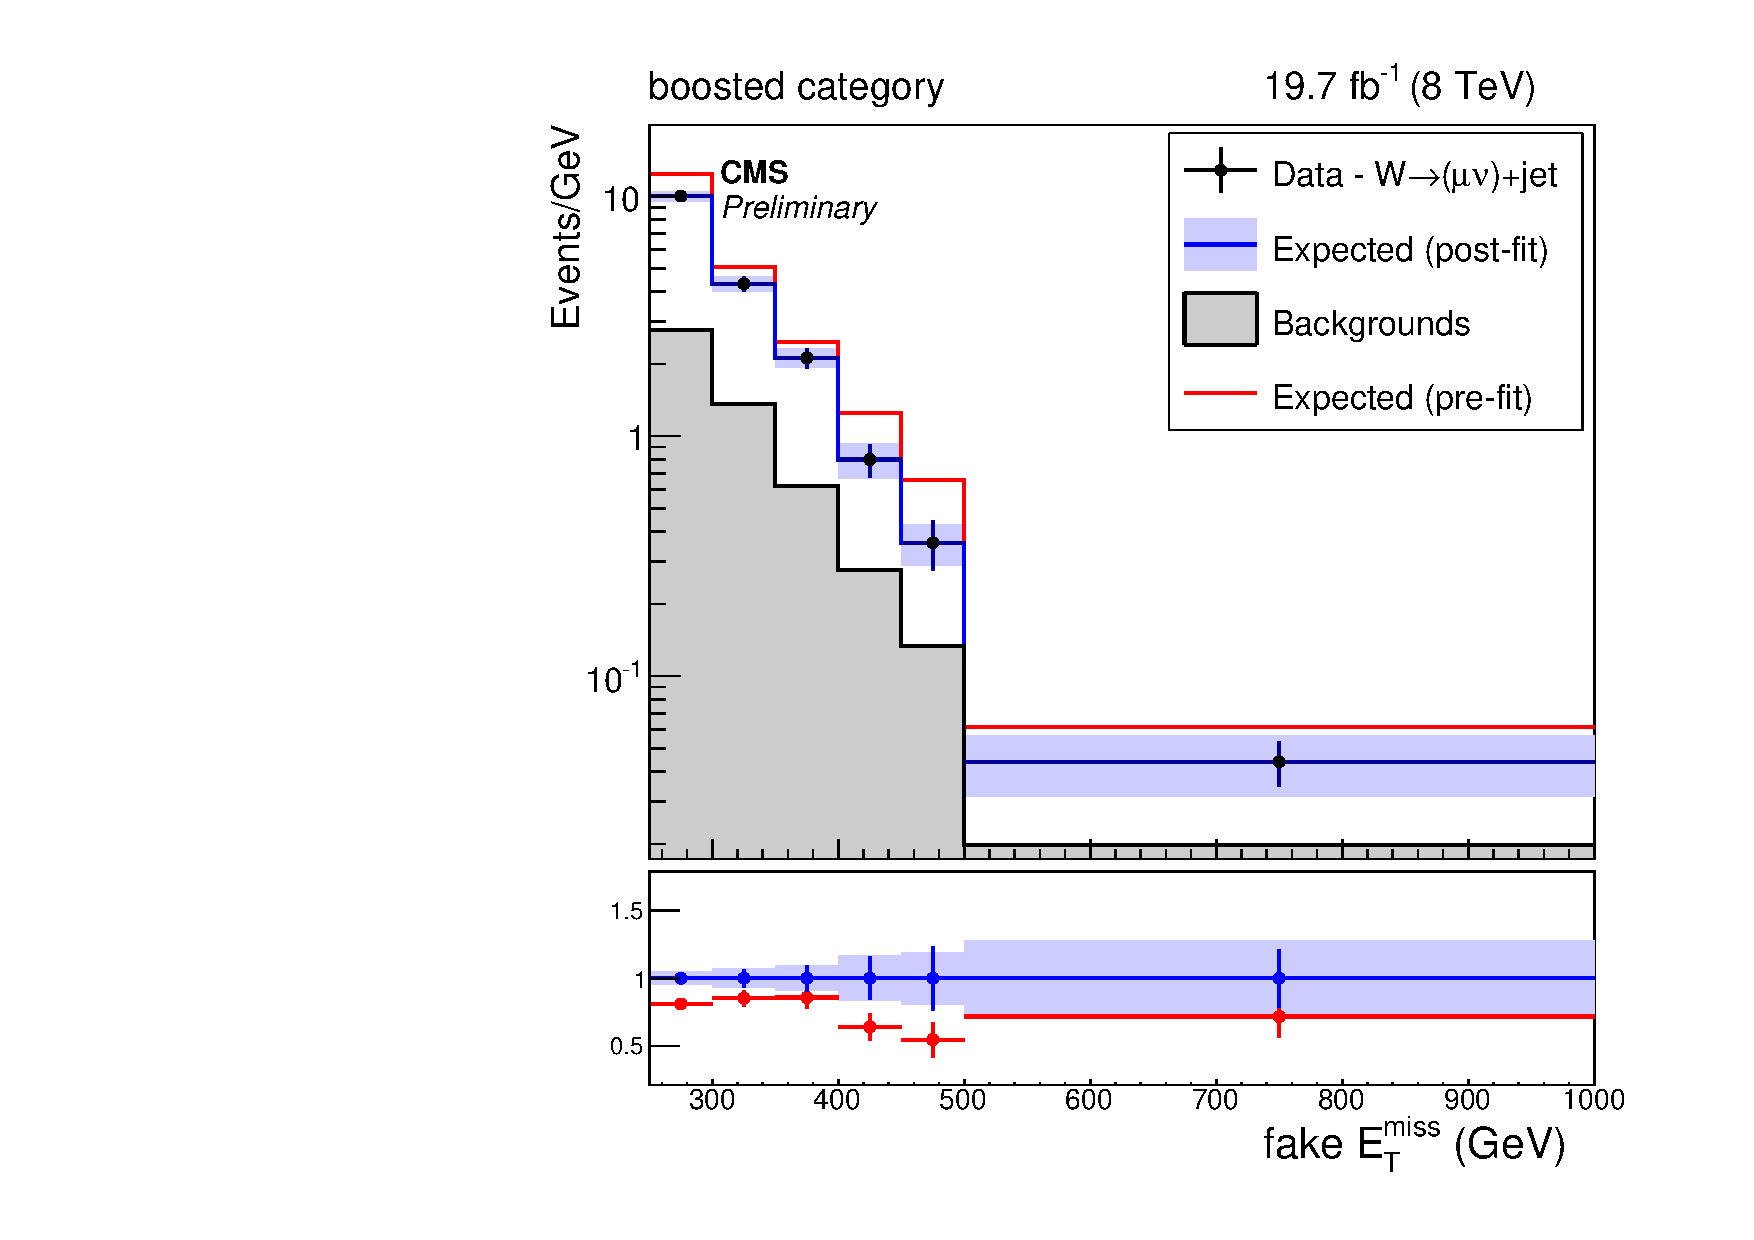
\includegraphics[width=0.32\textwidth]{fig/post_fit_wmn_boosted.pdf}\\
\end{center}
 \caption{Post-fit expected and observed (fake) \ETm distributions in the photon plus jet~(\cmsLeft), dimuon (middle) and single muon~(\cmsRight) 
 control regions from the parametric analysis. Each row, from top to bottom, shows the result of the fit in the monojet, resolved and boosted event categories 
 respectively. The red line represents the expected distribution before fitting to the control regions while the blue line shows the expectation after 
 the fit. In the the ratio, the blue and red points show the ratio of the observed data to the post-fit and pre-fit expectations 
 respectively. The blue bands indicate the statistical and systematic uncertainties from the fit.\label{fig:combined_fit_result_mbin} }
\end{figure}

\subsubsection{Single bin cut-and-count analysis}

The single bin  cut-and-count analysis has proven to be a robust style of analysis and frequently used in searches for new 
phenomena. It is however less sensitive than a shape-based analysis but may nevertheless be used as a 
cross-check of results. For the cut and count analysis, the \ETm shape is collapsed into a single bin with 
$\ETm> 500,~ 400, \textrm{and} 250$ GeV for the monojet, boosted and resolved event categories.
The threshold in the monojet category is chosen so that this analysis can also be directly compared to the DM 
interpretation results obtained in~\cite{monojet1}. For the other two categories, the threshold is relaxed due 
to the limited statistics avialable. 

The same likelihood as equation~\ref{eqn:candclh} 
is used to derive the correction for the V+jets backgrounds but with the bin index suppressed. The use of a single 
bin then removes both the power of the shape-based analysis the use of a functional form for deriving the corrections.
Table~\ref{tab:sbincandc} shows the expected yields from SM backgrounds, after applying the corrections, in 
each of the three event categories.

\begin{table*}[htbp]
  \begin{center}
    \topcaption{Expected yields for SM backgrounds and observed data for the cut-and-count analysis in the signal 
	region for each of the three event categories. The total uncertainty on the $\Zvvjets$ and $\Wlvjets$ components 
due to the statisitcal and systematic uncertainties due to the use of the three control regions is included. \emph{\textcolor{red} {Data are blind}}
      \label{tab:sbincandc}}
    \begin{tabular}{lccc}
      \hline
      \hline
      Expected Yields 		    & Boosted & Resolved & Monojet \\
      		 		    &($\ETm>$400 GeV) &($\ETm>$250 GeV) &($\ETm>$500 GeV) \\
      \hline
      \hline
      Z($\rightarrow \nu\nu$)+jets  & 117.2$\pm$9.4 (8\%)     & 445.6$\pm$20.7 (4.6\%) & 398.9$\pm$ 28.9 (7.3\%)  \\
      W($\rightarrow l\nu$)+jets    & 21.3 $\pm$3.5 (16.6\%)  & 293.9$\pm$23.0 (7.8\%) & 80.4 $\pm$ 4.9 (6.1\%) \\                
      Dibosons  		    & 23.2  & 36.5  & 7.4  \\           
      top  			    & 2.6   & 64.7  & 0.8  \\               
      Z($\rightarrow ll$)+jets      & 0.0   & 2.3   & 0.3  \\ 
      QCD		            & 0.0   & 34.2  & 0.0  \\ 
      \hline
      Total Backgrounds		    & 163.4 & 877.2 & 487.7  \\
      Data                          & X & X & X \\
      \hline
      \hline
    \end{tabular}
  \end{center}
\end{table*}


\subsubsection{Comparing the analysis}
The sensitivity of the analyses are compared by determining the expected 95\% CL upper limit on the branching ratio
of a Higgs boson with mass 125 GeV decaying invisibly. Additionally, the sensitivity is compared in the context of 
a effective field theory (EFT) by comparing the expected 90\% CL lower limit on the contact interaction scale, $\Lambda$, 
for a scalar contact interaction~\cite{Beltran:2010ww,Goodman:2010ku} as a function of the dark matter mass, $m_{DM}$. 
The limits are extracted using the combination of all three event categories. The comparison of the expected limits is 
given in Table~\ref{tab:compareanalyses}. 
 
\begin{table*}[htbp]
  \begin{center}
    \topcaption{Comparison of expected limits using the three alternate analyses.}
      \label{tab:compareanalyses}}
    \begin{tabular}{lr|ccc}
      \hline
      \hline
      	Expected limits	    & & Baseline & Parametric & Cut-and-count  \\
      \hline
       $ BR(H\rightarrow \textrm{invisibles})$, $m_{H}=125$ GeV  & &   &  & \\
       95\% CL upper limit				 & & 0.53  & 0.54 & 0.76\\
      \hline
       EFT scalar contact  $\Lambda$ (GeV) & &   &  & \\
       90\% CL lower limit			& $m_{DM}$ (GeV)&   &  & \\         
 
      & 1    				         & 448.6  & 452.3 & 424.1\\
      & 200  				 & 426.3  & 429.6 & 403.0\\
      & 400  				 & 377.8  & 380.9 & 357.7\\
      & 700  				 & 298.0  & 300.6 & 282.1\\
      & 1000 				 & 227.5  & 229.5 & 215.6\\
      
      \hline
      \hline
    \end{tabular}
  \end{center}
\end{table*}


The comparison shows that the baseline and parametric analyses perform equally well for a Higgs signal. 
This is expected due to the fact that for this signal, the monojet category is the most performing and for this category. 
In this category, the signal populates the lower end of the distribution and due to the large number of 
events in the photon control region, the systematic uncertainty (largely from the Electroweak corrections to the ratio of the differential 
cross-section between the photon and Z) dominates in this region.
The statistical component of the uncertainty, which is treated differently between the two, is therefore less relevant for the Higgs signal. 
For the EFT model, the parametric analysis performs slightly better than the baseline due to the fact that the signal for this model 
populates the higher end of the \ETm spectrum at which the parametric method is expected to constrain the V+jets backgrounds.
The cut-and-count analysis can be directly compared to the scalar EFT results obtained in ~\cite{monojet1}. This analysis shows roughly 8\% 
improvement in terms of the expected lower limit on $\Lambda$. This is due to the inclusive of the photon plus jet control region which 
significantly reduces the uncertainty on the $\Zvvjets$ background.

 
